\subsection{Evaluation der Genauigkeit der Positionsermittlung mit unterschiedlichen Diensten}

  \begin{figure}[h]
    \begin{center}
    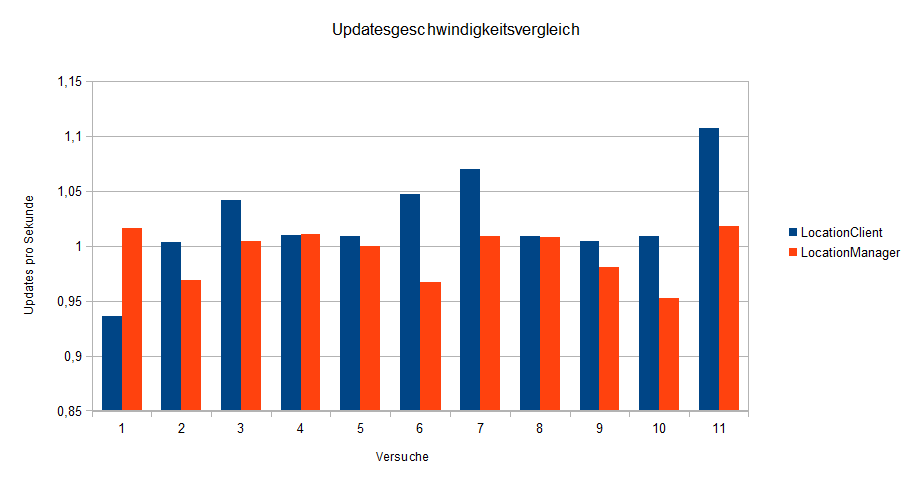
\includegraphics[width=1.0\textwidth]{4-Technische_Loesungen/4-1-Positionsermittlung/Data/updates_per_second_bigger.png}
    \end{center}
     \caption{Updates pro Sekunde}
     \label{fig: picUdates}
  \end{figure}
	
	\begin{figure}[h]
    \begin{center}
    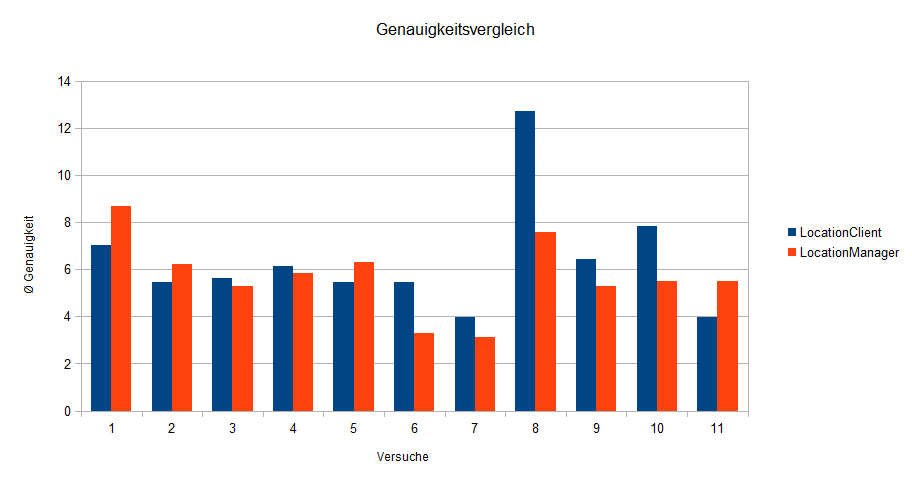
\includegraphics[width=1.0\textwidth]{4-Technische_Loesungen/4-1-Positionsermittlung/Data/accuracy_bigger.png}
    \end{center}
     \caption{Genauigkeit}
     \label{fig: picAccu}
  \end{figure}

Um LocationManager und LocationClient f�r unsere Zwecke vergleichen zu k�nnen, wurde ein Testprogramm entwickelt. Dieses sammelt in einer Datei jeweils in zwei separaten Activities unsere GPS-Messdaten. Je eine Activity verwendet dabei den LocationManager bzw. den LocationClient, um in regelm��igen Abst�nden Koordinaten, sowie deren approximierte Genauigkeit abzurufen und abzuspeichern. Das Experiment wird durchgef�hrt, indem eine Person mit dem Ger�t, auf dem das Testprogramm ausgef�hrt wird, eine m�glichst gerade Strecke abgeht. Zur optischen Darstellung der Ergebnisse wird aus den aufgezeichneten Koordinaten eine Linie (PolyLine\footnote{\url{https://developer.android.com/reference/com/google/android/gms/maps/model/Polyline.html}}) gezeichnet. Zum Vergleich wird eine Luftlinie zwischen Anfangs- und Endpunkt gezogen. Die ausgewerteten Sensordaten werden im Anhang \ref{app} dargestellt.

Der Genauigkeitswert ist hierbei folgenderma�en definiert: Um die ermittelte Position wird ein Kreis mit der ermittelten Genauigkeit als Radius gezeichnet. Der verwendete Dienst erstellt nun um die von ihm ermittelte Position einen Kreis. Die tats�chliche Position des Ger�ts liegt mit einer 68-prozentigen Wahrscheinlichkeit innerhalb dieses Kreises \footnote{\url{http://developer.android.com/reference/android/location/Location.html}}.
Es gilt, je kleiner der Kreis, desto genauer die Messung. 
In diesem Experiment wurden Versuche mit jeweils verschiedenen Ger�ten, Witterungsbedingungen und an unterschiedlichen Orten durchgef�hrt. Hierbei sollte untersucht werden, wie gut sich die jeweiligen Dienste unter unterschiedlichen Bedingungen schlagen. Die Ergebnisse sind im Anhang \ref{app} zu finden. Bei Genauigkeit und Updates pro Sekunde wurde jeweils das arithmetische Mittel der aufgezeichneten Daten eines Versuches eingetragen.
	  

Die Auswertung der Daten ergab, dass die Genauigkeit des LocationManagers in sechs von elf Versuchen pr�ziser war als die des LocationClients (siehe Graph \ref{fig: picAccu}). Im Bezug auf Updates pro Sekunde lieferte der LocationClient in neun von elf Versuchen die besseren Ergebnisse (siehe Graph \ref{fig: picUdates}).

Mit mobilen Endger�ten erzeugte Positionsdaten haben meist eine Genauigkeit von 2 bis 15 Metern. Dabei sind die Ergebnisse in offenem Gel�nde besser, als in engen Gassen \cite{gpsacc}. Befindet sich das Ger�t innerhalb eines Geb�udes sind die Ergebnisse unbrauchbar. Beides wurde durch die im Zuge der Evaluation durchgef�hrten Experimente best�tigt. Zus�tzlich hat auch die Witterung Einfluss auf die Genauigkeit der GPS-Positionen. Da beim Testen der entwickelten Anwendungen Ungenauigkeiten von f�nf oder mehr Metern als extrem st�rend empfunden wurden, k�nnen solche Spiele nur auf einem gen�gend gro�en, offenen Gel�nde gespielt werden. Die Updategeschwindigkeit von etwa einem Update pro Sekunde hat sich als ausreichend erwiesen, falls sich alle Mitspieler mit Schrittgeschwindigkeit bewegt haben. Gleichzeitig konnten die Spieler sich nicht schnell bewegen, da sie in regelm��igen Abst�nden auf ihr Handy schauen mussten.

\subsection{Entscheidung}
Genauigkeit ist in diesem Projekt ein wichtiger Faktor, vor allem im Bezug auf Kollisionen mit anderen Spielern und virtuellen Objekten. Da in diesem Projekt Mehrspieler-Spiele realisiert wurden, ist auch die Updategeschwindigkeit ber�cksichtigt worden. 
%Die Versuche haben gezeigt, dass bez�glich der Genauigkeit zwischen den beiden Dienste kein statistisch signifikanter Unterschied festgestellt werden kann. 
Da die im Zuge dieses Projekts entwickelten Anwendungen zur Umgebungsdarstellung auf GoogleMaps zu\-r�ck\-grei\-fen (siehe Abschnitt \ref{kartendarstellung}), das sowohl Google-Play-Services, als auch eine konstante Internetverbindung ben�tigt, kann der LocationClient ohne Bedenken wegen dieser Abh�ngigkeiten und fehlender Abw�rts\-kom\-pa\-ti\-bi\-li\-t�t eingesetzt werden.
Da dieser zus�tzlich durch tendenziell geringere Zeitintervalle zwischen den gelieferten Werten einen fl�ssigeren Spielablauf erm�glicht, wird in diesem Projekt der LocationClient verwendet. 
 